\chapter{Experiments} \label{ch:experiment}

In this section, we present the experiments we conducted for our model along with the
corresponding results for each experiment.

\section{Training Results} \label{sec:training-results}

We found that the model fails to learn the target texture accurately when the distribution
of the set of scene descriptions used for generating the dataset does not match the set of
scene descriptions used at runtime during training. We attribute this failure mode to two
primary causes.

\begin{figure}
    \centering
    \caption{We present our results side-by-side with the ground truth albedo as generated by
    a procedural dirt texture generator $\mathcal{G}_0$. The dataset this model was trained on
    contains images of cars rendered only from one side with a constant elevation angle. This
    causes the model to not learn patches that weren't visible in the whole dataset.}
    \label{fig:results-albedo}
    \vspace{0.2in}
    \begin{subfigure}[t]{0.4\linewidth}
        \centering
        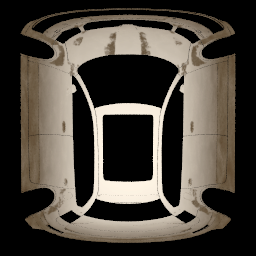
\includegraphics[width=\linewidth]{graphics/results_0_albedo.png}
        \caption{Target albedo}
    \end{subfigure}
    \begin{subfigure}[t]{0.4\linewidth}
        \centering
        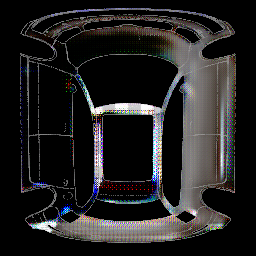
\includegraphics[width=\linewidth]{graphics/results_1_albedo.png}
        \caption{Model output}
    \end{subfigure}
\end{figure}

\begin{figure}[t]
    \centering
    \caption{We render the albedo-maps from Figure~\ref{fig:results-albedo} onto its corresponding
    car mesh and compare to the ground truth images.}
    \label{fig:results}
    \vspace{0.2in}
    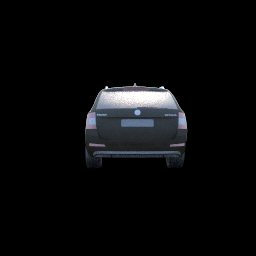
\includegraphics[width=.19\linewidth]{graphics/results_1_target.png}
    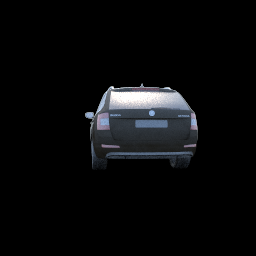
\includegraphics[width=.19\linewidth]{graphics/results_2_target.png}
    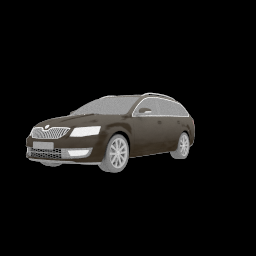
\includegraphics[width=.19\linewidth]{graphics/results_3_target.png}
    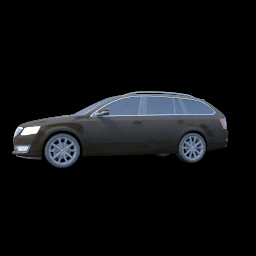
\includegraphics[width=.19\linewidth]{graphics/results_4_target.png}
    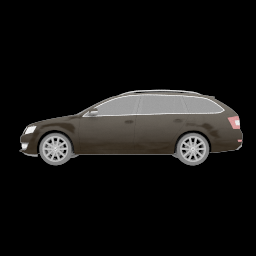
\includegraphics[width=.19\linewidth]{graphics/results_5_target.png}
    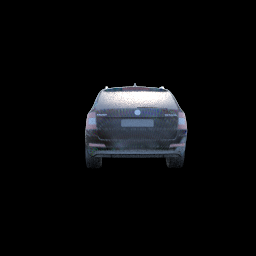
\includegraphics[width=.19\linewidth]{graphics/results_1_model.png}
    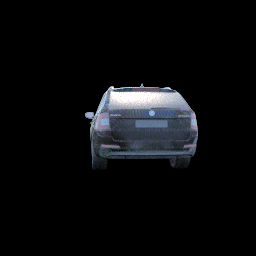
\includegraphics[width=.19\linewidth]{graphics/results_2_model.png}
    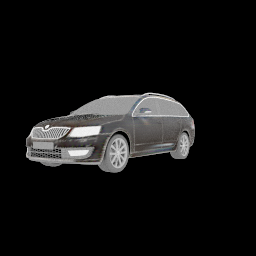
\includegraphics[width=.19\linewidth]{graphics/results_3_model.png}
    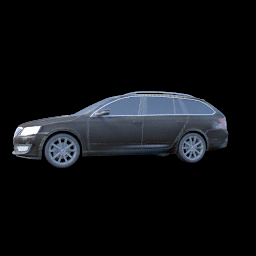
\includegraphics[width=.19\linewidth]{graphics/results_4_model.png}
    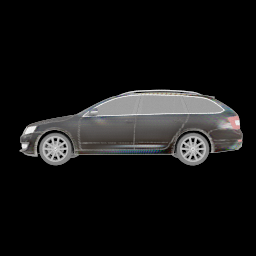
\includegraphics[width=.19\linewidth]{graphics/results_5_model.png}
\end{figure}

\begin{itemize}
\renewcommand\labelitemi{--}
    \item The discriminator learns to distinguish between the real and fake images using
        the discrepancy in the statistics of the scene description that is used to render it
        instead of using the generator output. We refer to this failure mode as discriminator
        \emph{mode collapse}.
    \item A batch size of $1$ prevents the model from passing useful gradients to the network
        weights due to lack of feature overlap between real and fake images at each iteration.
\end{itemize}

In order to address both of these issues, we elect to train the network by specifying the
scene description for each image using the scene description of the training images: at each
training iteration of the discriminator, an output from the generator is computed and applied
to the same scene as in the training image. The discriminator computes the GAN-loss on this
pair of real and fake images. Throughout this training procedure, the only difference the
discriminator observes between the pair of fake and real input images is the texture applied
to the cars.

This approach allows us to determine a baseline for whether our model is capable of learning
the target texture provided no ambiguity on what the discriminator can use to distinguish
real images from fake images.

\section{Ablation Study}

As mentioned in the previous section, our model does not train well unless the input image
scene description is shared between the real and fake images. We recognize that this
constraint prevents us from training our model on anything beyond the synthetic dataset we
generated for training purposes. If we hope to generalize our model for real image datasets
in the future, determining the model's robustness to non-matching scene-descriptions is
crucial. In this section, we present results from training our model after relaxing the
"matching scene description" constraint in a variety of controlled situations as a measure
of stress-testing our model's robustness.

\subsection{Camera Pose Distribution}

\begin{figure}
    \centering
    \caption{Increasing the noise $\epsilon$ in the pose estimation during training
        preserves the quality of the textures learned by the model. However, if the
        model and dataset pose distributions are non-overlapping, the discriminator
        experiences \emph{mode collapse}.}
    \label{fig:pose-vary-1}
    \vspace{0.2in}
    \begin{subfigure}[t]{0.19\linewidth}
        \centering
      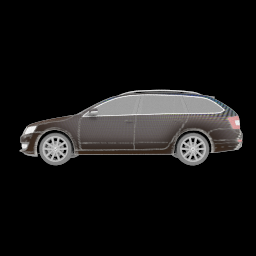
\includegraphics[width=\linewidth]{graphics/pose_1.png}
        \caption{$\epsilon < 1^\circ$}
    \end{subfigure}
    \begin{subfigure}[t]{0.19\linewidth}
        \centering
       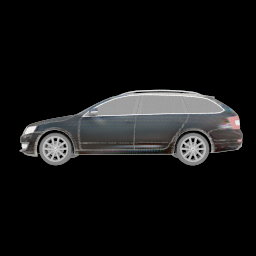
\includegraphics[width=\linewidth]{graphics/pose_2.png}
        \caption{$\epsilon < 2^\circ$}
    \end{subfigure}
    \begin{subfigure}[t]{0.19\linewidth}
        \centering
       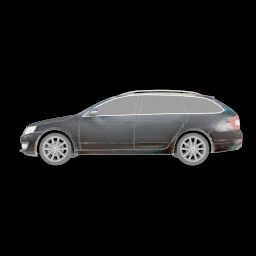
\includegraphics[width=\linewidth]{graphics/pose_5.png}
        \caption{$\epsilon < 5^\circ$}
    \end{subfigure}
    \begin{subfigure}[t]{0.19\linewidth}
        \centering
        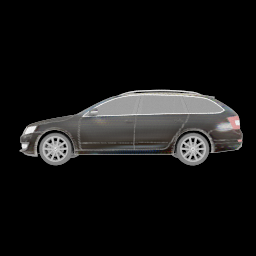
\includegraphics[width=\linewidth]{graphics/pose_10.png}
        \caption{$\epsilon < 10^\circ$}
    \end{subfigure}
    \begin{subfigure}[t]{0.19\linewidth}
        \centering
        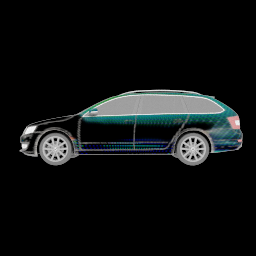
\includegraphics[width=\linewidth]{graphics/pose_diff.png}
        \caption{No overlap}
    \end{subfigure}
\end{figure}

We discussed the technical limitations that require us to train with a batch size of $1$
in Section \ref{training-process}. As a result we are not able to benefit from gradient averaging
used in deep learning models which decrease the volatility of the gradient at each iteration. If
at each iteration, the discriminator observes vastly different fake and real images, the
discriminator's task becomes more complex as it will have to learn to ignore the pose variation
of the cars before learning to label images using the texture observed on the car surfaces.

However, having perfect estimation of the camera pose from a real image is not realistic. At
best, we can get a noisy estimate of the camera pose. To investigate how much noise in camera
pose estimation the model can tolerate and what the effect is on model convergence speed and
the quality of the learned textures, we conduct several experiments where we perturb the camera
pose loaded from the training image scene by some random uniform noise. The results for this
experiments are shown in Figure~\ref{fig:pose-vary-1}. The figure shows that errors of up to 10
degrees in the pose estimation still allow the model to learn a reasonable texture-map. However,
the training time for the model increases as the noise increases.

In order to confirm our assumptions stated earlier, we experiment with a setup where the
distribution of the camera poses between the real and fake images is completely independent and
non-overlapping. If our assumption about the discriminator's \emph{mode collapse} as explained in
Section \ref{sec:training-results} is correct, this model should fail to learn a reasonable
texture-map. Unsurprisingly, this model does not learn a reasonable texture-map as shown in
Figure~\ref{fig:pose-vary-1}, likely because the discriminator learns the difference in camera
pose distributions between the real and fake image sets.

\subsection{Environment Map Distribution}

\begin{figure}
    \centering
    \caption{Varying the environment map distribution affects the quality of the outputs of our
        model. If we train a network with non-matching environment maps sampled from
        the training distribution, we learn a reasonable texture as shown in
        Figure~\ref{fig:pose-vary-sim}. Unfortunately, using environment maps sampled from a
        different distribution leads to \emph{mode collapse}.}
    \label{fig:pose-vary-1}
    \vspace{0.2in}
    \begin{subfigure}[t]{0.24\linewidth}
        \centering
        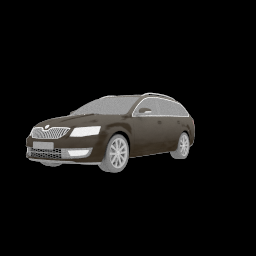
\includegraphics[width=\linewidth]{graphics/envmap_target.png}
        \caption{Target Image}
    \end{subfigure}
    \begin{subfigure}[t]{0.24\linewidth}
        \centering
       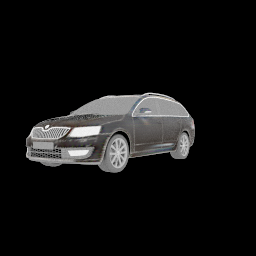
\includegraphics[width=\linewidth]{graphics/results_3_model.png}
        \caption{Same dist, match}
    \end{subfigure}
    \begin{subfigure}[t]{0.24\linewidth}
        \centering
        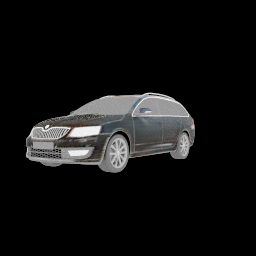
\includegraphics[width=\linewidth]{graphics/envmap_sim.png}
        \caption{Same dist, no match}
        \label{fig:pose-vary-sim}
    \end{subfigure}
    \begin{subfigure}[t]{0.24\linewidth}
        \centering
        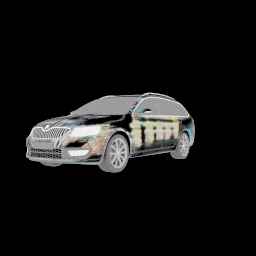
\includegraphics[width=\linewidth]{graphics/envmap_diff.png}
        \caption{Different dist, no match}
    \end{subfigure}
\end{figure}

The overall brightness, contrast, and white balance of a rendered image is heavily affected
by the lighting parameters of the scene. We observe that the choice of environment map
distributions has the highest amount of effect on the network's ability to learn the target
texture.

For the environment map ablation study, we experiment with two general setups for which we
report our findings.

\subsubsection{Non-matching samples drawn from the same distribution}

At each iteration, we render the fake image by randomly sampling an environment map
configuration that does not match the configuration loaded from the scene description of the
real image. However, we sample the configuration from the same distribution as the real image
dataset. Doing so allows us to check whether there are any effects other than discriminator
\emph{mode collapse}. The results of this experiment show that the model successfully learns
the target texture, albeit with a slower convergence rate, which is expected.

\subsubsection{Samples drawn from a different distribution}

In this setup, we draw the samples of environment map configurations for the fake and real
images from a mutually exclusive distribution; each set is rendered using completely different
environment maps. Unfortunately, in this experiment the model fails to converge on a realistic
surface texture-map generator. This result is likely due to \emph{mode collapse}.

The inability to learn a texture-map due to inaccuracy of the environment map makes it difficult
for us to easily extend our model to train on real images. Unless we have a good estimation
of the set of environment maps used in the dataset, the model will fail to converge on real images.

\section{GAN Loss function}

Different GAN loss functions have vastly different results when trained for our model.
Figure~\ref{fig:gan-results} shows the comparative results between the convergence speed and
resultant textures between vanilla GAN loss, WGAN loss with gradient penalty, and LSGAN loss
functions respectively. The WGAN with gradient penalty shows the best results visually, while the
LSGAN model fails to learn a reasonable texture-map.

\begin{figure}
    \centering
    \caption{Different GAN loss functions produce different results when training our model. From
        left to right, we show our results for vanilla GAN, WGAN w/ gradient penalty, and LSGAN.
        The LSGAN model falls into \emph{mode collapse}.}
    \label{fig:gan-results}
    \vspace{0.2in}
    \begin{subfigure}[t]{0.3\linewidth}
        \centering
       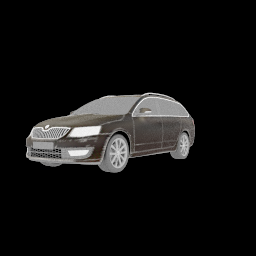
\includegraphics[width=\linewidth]{graphics/gan_vanilla.png}
        \caption{Vanilla GAN}
    \end{subfigure}
    \begin{subfigure}[t]{0.3\linewidth}
        \centering
      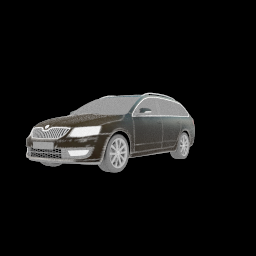
\includegraphics[width=\linewidth]{graphics/gan_wgangp.png}
        \caption{WGAN w/ gp}
    \end{subfigure}
    \begin{subfigure}[t]{0.3\linewidth}
        \centering
      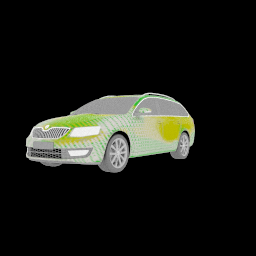
\includegraphics[width=\linewidth]{graphics/gan_lsgan.png}
        \caption{LSGAN}
    \end{subfigure}
\end{figure}